\chapter{Grundlagen}


% !TeX spellcheck = en_US
\section{Unscharfe Daten und Fuzzy-Logik}
In dem normallen Alltag eines Menschen werden ständig Aussagen über Ereignisse getroffen. Diese Aussagen können möglichst exakt sein, oder auch nicht. In manchen Situationen werden solche genannt, die für den Menschen adäquat ein Ereignis beschreiben. Man würde zum Beispiel sagen, dass es gerade sehr stark regnet, oder es sehr heiß ist. Diese Information kann von dem menschlichen Gehirn angemessen vearbeitet werden. Maschinen, wie Komputern, sind jedoch nicht mit dieser Funktionalität ausgestattet. Die sogenannten unscharfe Daten müssen somit anders repräsentiert werden, damit auch Maschinen diese verarbeiten können. Auf dieser Weise können wir den Vorteil der Maschinen gegenüber Menschen ausnutzen - ihre große Kapazität und die Möglichkeit komplexere Strukturen und Systeme darzustellen. In diesem Kapitel wird eine Erweiterung der klassischen Logik vorgestellt, die es den Komputern ermöglicht, unscharfe Daten darzustellen und darauf Operationen durchzuführen. Diese Logik ist als Fuzzy-Logik bekannt.

\section{Fuzzy-Logik}\label{fuzzy_logik}

%Eine Menge beschreibt ein Zusammenhang von Elementen, oder Objekte. Jedes Element erf�llt eine bestimmte Eigenschaften. In der klassischen Mengenlehre geh�rt ein Element entweder vollst�ndig oder nicht.

In der Literatur bezeichnet man die präzise Erfassung von unscharfen Daten als Fuzzy-Logic. Fuzzy-Logic unterscheidet sich von der klassischen Mengenlehre darin, dass Elemente graduell einer Menge gehören und nicht nur bivalente Zugehörigkeit erweisen können.

Zum Verdeutlichen betrachten wir die Menge M der reellen Zahlen, die viel größer als 1 sind.
%\cite{CIKruse:15}

\begin{align}
\centering
M = \{ x \ |\ x \in \Re,\ x >> 1\}
\end{align}

Wird diese Menge M mit der klassischen Logik modelliert, ergibt sich die Problematik: Der Vergleich ``viel größer'' ist mathematisch nicht eindeutig definiert. Auf der Grafik \ref{class_dar} unten kann man die Modellierung mit der klassischen Logik sehen.

%Hier Graphik f�r die Set mit klassiche Darstellung viel gr��er als 1

\begin{figure}[htbp]
	\centering
	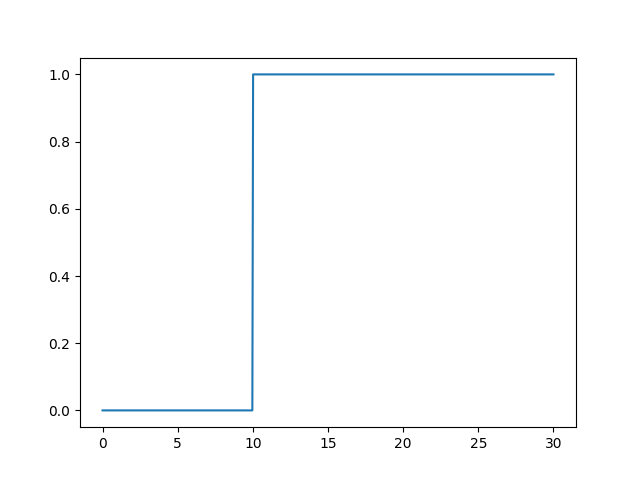
\includegraphics[scale=0.5]{images/classic_logic.png}
	\caption{``Viel größer als 1'' in der klassischen Logik}\label{class_dar}
\end{figure}

Aus der Abbildung \ref{class_dar} kann man feststellen, dass alle Werte kleiner als $10$ eine Zugehörigkeit von $0$ und solche größer oder gleich $10$ - eine Zugehörigkeit von $1$ besitzen. Diese Repräsentation entspricht jedoch die Realität nicht. Es ist eindeutig, dass $9.9$ als Wert schon größer als $1$ ist, aber der Abbildung \ref{class_dar} nach wird das nicht klar. Würde man diese Menge in der Fuzzy-Logik darstellen, ergibt sich folgende Abbildung.

% Hier Graphik f�r die Fuzzy-Set "viel gr��er als 1"
\begin{figure}[htbp]
	\centering
	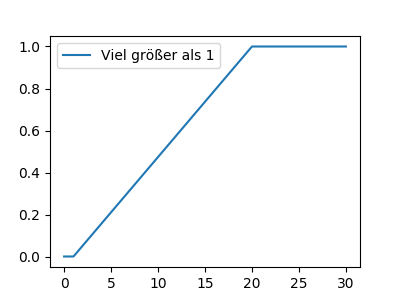
\includegraphics[scale=0.5]{images/fuzz_logic.png}
	\caption{``Viel größer als 1'' in der Fuzzy-Logik}\label{fuzzy_dar}
\end{figure}

Hier beschreibt die Ausbildung \ref{fuzzy_dar} genauer, wie die Zahlen im Vergleich zu $1$ stehen. Die Zugehörigkeit nimmt Werte zwischen $0$ und $1$. Zum Beispiel der Wert $10$ hat die Zugehörigkeit von ca. $0.5$ und für Werte größer als $20$ liefert die Funktion $\mu (x)$ einen Wert von $1$ (volle Zugehörigkeit).


\subsection{Fuzzy-Sets}\label{fs_section}%Eventuell hier beschreiben
Fuzzy-Sets, oder Fuzzy-Mengen, beschreiben in der Fuzzy-Logik Eigenschaften von Elementen. Die Idee ist, dass Elemente zu einem rationallen Wert einer Menge gehören, beziehungsweise eine Eigenschaften besitzen. In der Literatur wird folgende Definition für Fuzzy-Mengen gegeben \cite{CIKruse:15}:

\begin{definition}
	Eine Fuzzy-Menge oder Fuzzy-Teilmenge $\mu$ der Grundmenge $X$ ist eine
	Abbildung $\mu : X \rightarrow [0, 1]$, die jedem Element $x \in X$ seinen Zugehorigkeitsgrad $\mu(x)$ zu
	$\mu$ zuordnet. Die Menge aller Fuzzy-Mengen von $X$ bezeichnen wir mit $F(X)$. \cite{CIKruse:15}
\end{definition}

Mengen aus der klassischen Logik können als spezielle Fuzzy-Mengen aufgefasst werden. Also sind Fuzzy-Sets verallgemeinerte charakteristische Funktionen \cite{CIKruse:15}.

In der Praxis werden mehrere Arten von Fuzzy-Mengen entwickelt. Die bekanntesten davon sind Dreiecksfunktion, Trapezfunktion und Gaußfunktion. Ihre Namensgebung ergibt sich aus der Funktion, die sie berechnet. Drei Beispielfunktionen sind unten gegeben.

\begin{figure}[htbp]
	\centering
	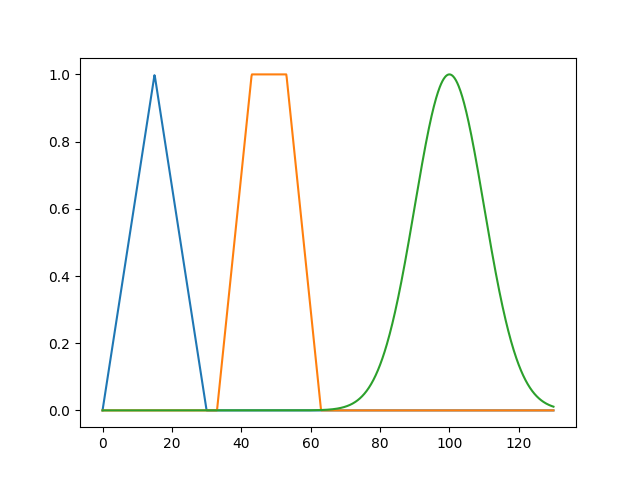
\includegraphics[scale=0.5]{images/mf_types.png}
	\caption{Dreiecks-, Trapez- und Gaußfunktion von Fuzzy-Mengen}\label{mf_types}
\end{figure}

Die Form einer Fuzzy-Menge ist durch ihre Funktion bestimmt. Die Berechnung der Dreiecksfunktion wird in \ref{dreieckfunc} .

\begin{equation}
\mu_{tri}(x) = \begin{cases}
\frac{x - a}{b - a} & \text{falls $a \leq x \leq b$}\\
\frac{c - x}{c - b} & \text{falls $b \leq x \leq c$}\\
0 & \text{sonst}
\end{cases}\label{dreieckfunc}
\end{equation}

Der Index der Funktion verdeutlicht, dass es sich um die Dreiecksfunktion handelt. Die Funktion hat drei Parametern $a, b$ und $c$, für die $a < b < c$ gelten muss. Die Dreiecksfunktion ist ein besonderer Fall der Trapezfunktion, wo die Punkte, bzw. Parametern, der oberen Grudseite gleich sind. Deswegen ist die Gleichung \ref{trap_mf} für die Trapezfunktion sehr ähnlich \cite{CIKruse:15}.

\begin{equation}
\mu_{trap}(x) = \begin{cases}
\frac{x - a}{b - a} & \text{falls $a \leq x \leq b$}\\
1 & \text{falls $b \leq x \leq c$}\\
\frac{d - x}{d - c} & \text{falls $c \leq x \leq d$}\\
0 & \text{sonst}

\label{trap_mf}
\end{cases}
\end{equation}

Die Glockefunktion ist, wie ihrer Name andeutet, eine Funktion, die die Form einer Glocke hat. Die Darstellung dieser Funktion ähnelt sich sehr der Gaußsche Funktion. Die Berechnung wird in \ref{bell_mf} gegeben. 

\begin{equation}
\mu_{bell}(x) = \frac{1}{1 + [(\frac{x - c}{a})^2]^b}
\label{bell_mf}
\end{equation}

Die letzte Funktion, die vorgestellt werden soll, ist die gaußsche Funktion. Die Formel wird öfters in der Statistik für Darstellung von Nominalverteilungen, aber auch in der Fuzzy-Logik, benutzt. Die Gaußfunktion ist in \ref{gauss_mf} gegeben \cite{CIKruse:15}:

\begin{equation}
\mu_{gauss}(x) = exp(\frac{-(x - m)^2}{s^2})
\label{gauss_mf}
\end{equation}

Die Parametern $m und q$ sind entsprechend der Mittelwert (Mittelpunkt) und die Abweichung von der Mitte, oder als $\sigma$ (Sigma) in der Statistik bekannt.




%[Fuzzy-Logik und Fuzzy-Control, Jörg Kahlert; Hubert Frank,]
%
%
%   [Fuzzy-Logik und Fuzzy-Control, Jörg Kahlert; Hubert Frank, Computational Intelligence]

\section{Operationen auf Fuzzy-Sets} \label{operatoren}
In dem vorherigen Unterkapitel \ref{fuzzy_logik} wurde die Fuzzy-Logik eingeführt, so wie auf die Repräsentation von Fuzzy-Mengen eingegangen. Um nun unscharfe Informationen verarbeiten zu können, wie Schlüsse daraus zu ziehen oder mehrere Fuzzy-Mengen zu kombinieren, brauchen wir eine Reihe von Operatoren. Da es um Mengen geht, eignen sich die Durchschnitt-, Vereinigung- und Komplementbildung aus der klassischen Logik gut. Im folgenden Kapitel werden die einzelnen Operationen beschrieben.
%\cite{} [Computational Intelligence]
\subsection{Durchscnitt}\label{AND}

In der klassischen Logik ist der Durchschnitt durch einen Logischen-UND eingesetzt. die Menge aller Elementen, die zu einer Menge $M_1$ und einer Menge $M_2$ gehören,  ist als Schnittmenge definiert. Gegeben seien die Mengen:

\begin{align}
M_1 = \{ x \ | \ x \in\Re, \ 1 \ \leq \ x \ \leq \ 3 \} 
\end{align}
\begin{align}
M_2 = \{ x \ | \ x \in\Re, \ 2 \ \leq \ x \ \leq \ 4 \} 
\end{align}

Der Durchschnitt der beiden Mengen ergibt sich aus:

\begin{align}
M_1 \cap M_2 = \{ x \ | \ x \in \Re, \ 2 \ \leq \ x \ \leq \ 3 \}
\end{align} 

Der UND-Operator lässt sich analog auf die Fuzzy-Mengen anwenden. Es wird die Fläche bestimmt, die für beide Mengen erfüllt ist. Aus methematischer Sicht sprechen wir von dem Minimum-Operator(MIN).

%\theoremstyle{definition}
\begin{definition}
	Seien $\mu_1$ und $\mu_2$ zwei Fuzzy-Mengen auf der Grundmenge $G$. Dann heißt:
	\begin{center}
		$\mu_1$ $\cap$ $\mu_2$ : $G$ $\rightarrow$ [0,1] $\text{mit}$ ($\mu_1$ $\cap$ $\mu_2$)($x$) $=$ MIN($\mu_1$($x$) , $\mu_2$($x$)) 
	\end{center}
	der \textbf{Durchschnitt} der Fuzzy-Mengen $\mu_1$ und $\mu_2$.
\end{definition} 

Zur Veranschaulichung wird unten die Grafik angegeben. Da sind zwei Fuzzy-Sets dargestellt. Die zwei Ausdrücke, die betrachtet werden, sind $mittlere$ und $hohe$ Temperatur. Der rote gestrichene Bereich stellt die Ergebnismenge dar.

\begin{figure}[htbp]
	\centering
	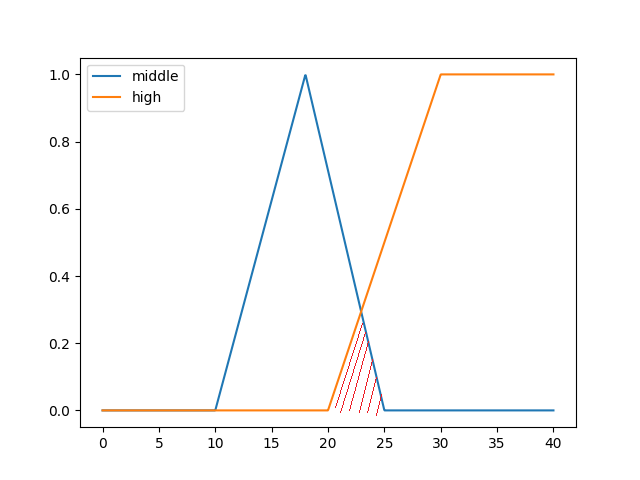
\includegraphics[scale=0.5]{images/und_high_middle_temp.png}
	\caption{Durchschnitt von zwei Fuzzy-Mengen (roter gestrichener Bereich)}\label{high_low_temp_intersection}
\end{figure}

%hier Grafik f�r die Mittlere und Hohe Temperatur mengen.


\subsection{Vereinigung}

Nehmen wir ganz einfach die Definition der Vereinigung aus der klassischen Mengenlehre:
\begin{center}
	$x$  $\in$ $M_1$ $\cup$ $M_2$ $\Leftrightarrow$ $x$ $\in$ $M_1$ $\vee$ $x$ $\in$ $M_2$
\end{center}

Ziemlich eindeutig und klar. Die Vereinigungsmenge enthält alle diese Elemente aus dem Grundbereich, die entweder in der Menge $M_1$ oder $M_2$ enthalten sind. Im nächsten Schritt wird dieser Operator an die Fuzzy-Mengen angepasst.

In der Mathematik ist dieser Operator als ODER-Verknüpfung angegeben. Die Anwendung der ODER-Operator auf Fuzzy-Mengen wird wie folgt dann definiert:

%\theoremstyle{definition}

\begin{definition}
	Seien $\mu_1$ und $\mu_2$ zwei Fuzzy-Mengen auf der Grundmenge $G$. Dann heißt:
	\begin{center}
		$\mu_1$ $\cup$ $\mu_2$ : $G$ $\rightarrow$ [0,1] $\text{mit}$  ($\mu_1$ $\cap$ $\mu_2$)($x$) $=$ $MIN$($\mu_1$($x$)), $\mu_2$($x$)) 
	\end{center}
	die $\textbf{Vereinigung}$ der Fuzzy-Mengen $\mu_1$ und $\mu_2$.
\end{definition}

Betrachten wir den selben Beispiel aus vorherigen Unterkapitel. Seien also wieder die Fuzzy-Mengen für \textit{``mittlere''} und \textit{``hohe''} Temperatur. Wenn wir den ODER-Operator auf die beiden Mengen anwenden, ergibt sich eine Ergebnismenge, die sich auf beiden Mengenflächen aufstellt. Dies wurde graphisch zunächst aufgezeichnet.

\begin{figure}[htbp]
	\centering
	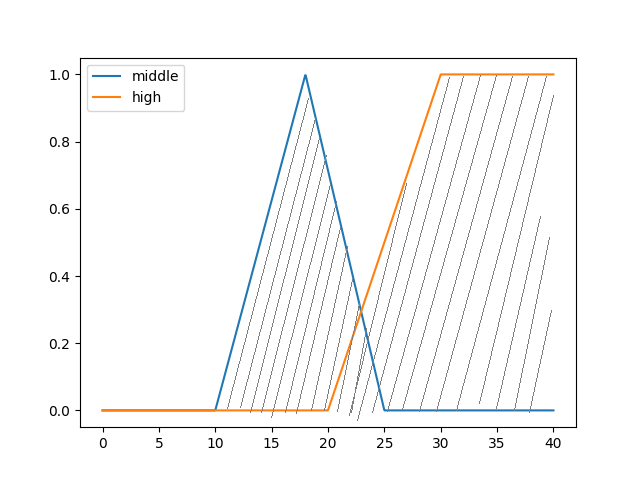
\includegraphics[scale=0.5]{images/oder_mid_high_temp.png}
	\caption{Union von Fuzzy-Mengen (gestrichener mit Blau Bereich)}
\end{figure}\label{high_low_temp_union}
% Hier Graphik f�r Oder verkn�pfung  

\subsubsection{Komplement}

Der dritte wichtige Operator ist das Komplement einer Menge. In der klassischen Mengenlehre ist dieser Operation ziemlich einfach anzuwenden. Der Operator beschreibt die Negation einer Aussage - zum Beispiel die Wahrscheinlichkeit eine 6 zu würfeln wäre $\frac{1}{6}$, die Gegenwahrscheinlichkeit, oder die Wahrscheinlichkeit etwas anderes als 6 zu würfeln wäre: (1 - $\frac{1}{6}$) = $\frac{5}{6}$. Das Komplement ist in der Fuzzy-Logik dann wie folgt definiert: 

\begin{definition}
	Sei $\mu$ eine Fuzzy-Menge auf der Grundmenge $G$. Dann heißt:
	\begin{center}
		$\mu^c$  : $G$ $\rightarrow$ [0,1] $\text{mit}$  ($\mu^c$)($x$) $=$ $1$ - $\mu$($x$)) 
	\end{center}
	die $\textbf{Vereinigung}$ der Fuzzy-Mengen $\mu_1$ und $\mu_2$.
\end{definition}

Zur Veranschaulichung die Menge \textit{hohe} Temperatur negiert. Die Negierung ist in der Graphik unten zu sehen.

%Hier Grafik f�r das Komplement-Beispiel

\begin{figure}[htbp]\label{not_high_temp}
	\centering
	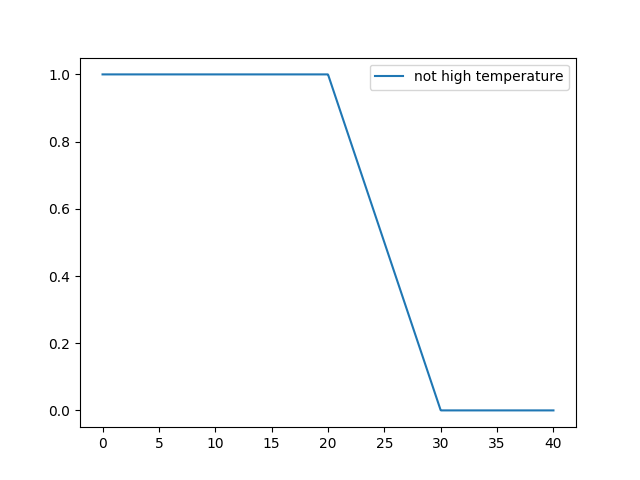
\includegraphics[scale=0.5]{images/not_high_temp.png}
	\caption{Komplement der Menge hohe Temperatur}
\end{figure}

\subsubsection{Zusammenfassung}

In diesem Unterkapitel \ref{operatoren} habe ich die drei wichtigsten Operatoren auf Fuzzy-Mengen vorgestellt. Neben den Grundverknüpfungen gibt es eine weitere Sammlung von Verknüpfungsoperatoren.

\begin{enumerate}
	\item Algebraisches Produkt: ($\mu_1$$\mu_2$) = $\mu_1$($x$) $\cdot$ $\mu_2$($x$)
	\item direkte Summe: ($\mu_1$ $\bigoplus$ $\mu_2$) = $\mu_1$($x$) + $\mu_2$(x) - $\mu_1$($x$) $\cdot$ $\mu_2$($x$)
	\item abgeschnittene Differenz: ($\mu_1$ $\sqfrowneq$ $\mu_2$) = MAX(0, $\mu_1$(x) + $\mu_2$(x) - 1)
	\item abgeschnittene Summe: ($\mu_1$ \^{+} $\mu_2$) = MIN(1, $\mu_1$(x) + $\mu_2$(x))
	\item ($\mu_1$$\dotminus$ $\mu_2$) = MIN($\mu_1$(x), 1 - $\mu_2$(x))
	\item ...
\end{enumerate}

Dies ist eine Vorbereitung auf die folgenden Kapiteln. Wir analysieren mehrere Fuzzy-Mengen und ziehen daraus bestimmte Schlüsse. Ein Beispiel dafür wäre: Wenn eine Tomate rot ist, dann ist die reif. Folgende Logische Aussagen können sehr einfach mit Fuzzy-Logic modelliert werden. In der Literatur taucht die Name Fuzzy-Regeln. Diese können dann zusammengestellt werden, um Fuzzy-Regel-Systeme aufzubauen. Das nächste Unterkapitel \ref{fuzzy_systeme} stellt Fuzzy-Systeme vor. 

\section{Fuzzy-Systeme}\label{fuzzy_systeme}

Ein Fuzzy-System, auch Fuzzy-Regler oder Fuzzy-Inferenz-System, ist ein bekannter Framework basierend auf Fuzzy-Mengen-Theorie, Fuzzy Wenn-Dann-Regeln und Fuzzy Reasoning. Konzeptionell besteht ein Fuzzy-System aus drei Grundteile - die Regelbasis, welche die Wenn-Dann-Regeln beinhaltet; die Datenbank(oder das Wörterbuch), die alle Zugehörigkeitsfunktionen definiert; und der Entscheidungmechanismus, wer die Inferenz durchführt und eine angemessene Schlussfolgerung erkundet.   

Folglich werden zwei Arten von Fuzzy-Systeme erläutert - Mamdani- und Takagi-Sugeno-Kang-Systeme.

\subsection{Mamdani-Regler}

Der Mamdani-Regler wurde im Jahr 1975 von Mamdani auf der Basis einer Veröffentlichung von Zadeh aus der Anfang der siebziger Jahren entwickelt. 

Der Mamdani-Regler ist eine endliche Menge von Wenn-Dann-Regeln $R$ der Form:
\begin{equation}
R: \text{If } x_1 \text{ is } A_1 \text{ and ... and } x_n \text{ is } A_n
\text{ then } y^\prime \text{ is } B
\end{equation}

In der Regel sind $x_1$, ..., $x_n$ die Eingangsgrößen und $y^\prime$ die Ausgabe. $A_i$ und $B$ sind  linguistischen Werte. Jede Regel besteht aus zwei Teilen - Prämissen und Konklusionen. Jede Vorbedingung untersucht spezifische Eigenschaften. Es wird geprüft, ob der Eingangwert diese Eigenschaften erfüllt. Anhand diese Merkmale schließt sich eine Konklusion. 

Sei $W$ die Menge aller linguistischen Konklusionen $B_i$, so dass $B_1, \dots, B_m \in W$ gilt. Der Regler kann als eine n-Stellige Funktion mit $f: \mathbb{G^n} \mapsto W$ dargestellt werden. Die Funktion ordnet eine Eingabe zu einem linguistischen Term $B_i$.

\begin{equation}
f(x_1, ..., x_n) \approx 
\left\{
\begin{array}{ll}
B_1 & \mbox{ falls } x_1 \mbox{ is } A_1^{(1)} \mbox{ und ..., und } x_{n} \mbox{ is } A_n^{(1)}\\
\vdots \\
B_{m} & \mbox{ falls } x_1 \mbox{ is } A_1^{(m)} \mbox{ und ... und } x_{n} \mbox{ is } A_n^{(m)}
\end{array}
\right.
\end{equation}

In der Funktion gibt es genau so viele Ausgaben, wie es Regeln gibt - $m$.

Mit einem Mamdani-Regler können viele Probleme aus der reellen Welt definiert werden. Als kleines Beispiel eignet sich die Farben der Tomaten. Wir betrachten die Farbe als Eingabe. Die Ausgabe würde uns sagen, wie reif eine Tomate ist. Wir teilen unsere Eingangsgrößen in drei Farben: rot, gelb und grün. Daraus lassen sich entsprechend 3 Fuzzy-Mengen definieren. Als Ausgabe wird die Reife einer Tomate bestimmt. Das Ergebnis kann in drei Mengen anfallen: reif, halbreif oder unreif. Auf dieser Weise haben wir ein Mamdani-Fuzzy-Model, das aus 3 Fuzzy-Sets und aus 3 Regeln besteht. Die Regelbasis sieht wie folgt aus:

\begin{itemize}
	\item $R_1$: if x is rot, then y is reif.
	\item $R_2$: if x is gelb, then y is halbreif.
	\item $R_3$: if x is grün, then y is unreif.
\end{itemize}

Eine Tabelle für die Fuzzy-Relationen ist unten gegeben

\begin{table}\label{tomato:1}
	\centering
	\begin{tabular}{c|c c c}
		
		x \diagdown \ y & \ unreif & \ halbreif & \ reif \\ [0.5ex]
		\hline
		grün & 1 & 0 & 0 \\ 
		gelb & 0 & 1 & 0\\
		rot  & 0 & 0 & 1\\
		
	\end{tabular}
	\caption{Beispiel für Tomaten}
	
\end{table}

Wie man sieht die Tabelle ist ziemlich einfach zu lesen, wenn die Tomate grün ist, wird immer angenommen dass sie unreif ist. Man könnte entsprechend die Fuzzy-Mengen aus der Konklusion verfeinern. Das würde bedeuten, dass die Mengen sich überlappen. Unsere Tabelle könnte dann wie Tabelle \ref{table:1} aussehen:

\begin{table}
	\centering
	\begin{tabular}{c|c c c}
		
		x \diagdown \ y & \ unreif & \ halbreif & \ reif \\ [0.5ex]
		\hline
		grün & 1 & 0.5 & 0 \\ 
		gelb & 0.3 & 1 & 0.3\\
		rot  & 0 & 0.5 & 1\\
		
	\end{tabular}
	\caption{Beispiel für Tomaten}
	\label{table:1}
\end{table}

Abhängig davon wie man die Ausgangsmengen definiert, wie weit die Mengen überlappen, ergibt sich eine unterschiedliche Interpretation der Werte. Je mehr Fuzzy-Sets für eine Größe(Maß) definiert sind, desto besser könnte ihr Zustand repräsentiert werden. Mit der Anzahl der Fuzzy-Sets steigt die Komplexität eines Systems proportional.

Den oberen kleinen Beispiel zeigt wie einfach Mamdani-Modelle zu modellieren sind. Mamdani-Reglern finden in der Praxis öfters Einsetzung.

\section{Takagi-Sugeno-Kang-Modell} \label{TSK}

Das Takagi-Sugeno-Kang-Modell ist dem Mamdani-Modell sehr ähnlich. Der Unterschied erweist sich in der Konklusion. TSK-Regler verwenden Regeln der Form:

\begin{align}
R: \text{ If } x_1 \text{ is } \mu_R^{(1)} \text{ and \ldots and } x_n \text{ is } \mu_R^{(n)} \text{ then } y = f_R(x_1,\ldots,x_n).
\end{align}}

In den Prämissen der beiden Fuzzy-Systeme liegt kein Unterschied. Die Besonderheit des TSK-Modells liegt in der Konklusion. Da steht eine lineare Funktion, anstatt eine Fuzzy-Menge. In der Konklusion kann jede beliebige Funktion $f$ mit belibiger Eingabe berechnet werden. Die Form der linearen Funktion ist in \ref{lin_func} gegeben:
\begin{align}
f(x_1, \ldots, x_n) = p_0 + p_1\cdot x_1 + \ldots + p_n\cdot x_n,
\label{lin_func}
\end{align}
$p_0, \ldots, p_n$ sind die Parametern der Konklusionsfunktion. Für geeignet ausgewählte Parameterwerte beschreibt das TSK-Modell eine belibige mathematische Funktion, dies kann z.B. die Quadratfunktion sein. Für den Fall, dass die Parametern $p_1, \ldots p_n$ den Wert 0 haben, erhält man einen Mamdani-Modell mit scharfer Ausgabe. Solche Modelle heißen in der Literatur auch \textbf{zero-order Sugeno-Fuzzy-Modelle} \cite{SCTemassi:01, NFMBothe:98, NFSC:97}.
Als Beispiel kann folgende Regelbasis betrachtet werden:
\begin{align*}
&R_1: \text{ If } x \text{ is ``sehr klein'' then } y = 0\\
&R_2: \text{ If } x \text{ is ``klein'' then } y = 1\\
&R_3: \text{ If } x \text{ is ``groß'' then } y = 2\\
&R_4: \text{ If } x \text{ is ``sehr groß'' then } y = 3. \\
\end{align*}
Die Fuzzy-Sets sind ``sehr klein'', ``klein'', ``groß'' und ``sehr groß'' und die Ergebnisswerte entsprechend \textit{0, 1, 2 und 3}.

\subsubsection{Fuzzifizierung und Defuzzifizierung}\label{FDF} 

Der Vorgang eines Modells zerlegt sich in zwei Teilen - Fuzzifizierung und Defuzzifizierung. Der erste Begriff beschreibt den Prozess für die Evaluierung der Eingangswerte in Fuzzyinferenzsysteme. Es gibt mehrere Evaluierungsmethoden, beziehungsweise Fuzzifizierungsmechanismen, wie zum Beispiel die Gaußsche Funktion (\ref{fs_section}). Der zweite Begriff bezeichnet die Vorgehensweise bei der Berechnung der Ausgabe, oder Inferenz, eines Fuzzy-Systems. Die Reihenfolge der beiden Prozesse ist somit bestimmt. Da im vorrigen Kapitel schon Beispiele für Fuzzifizierungsverfahren vorgestellt werden, wird demnächst in den unterschiedlichen Arten von Defuzzifizierung eingestiegen.

Bei der Regelaktivierung unterscheidet man zwei Fällen. Wenn die Eingabe eine volle Zugehörigkeit zu einer Fuzzy-Menge ergibt, dann liefert das Modell ganz normal den Wert der entsprechenden Konklusionsfunktion. Bei partielle Aktivierung mehreren Regeln ergibt sich das Inferenzergebnis aus einem spezifischen Verfahren. Dafür werden bestimmte Inferenzmethoden angewendet, zum Beispiel das Center of Gravity, oder Center of Area. Einige dieser Methoden werden inden folgenden Unterkapiteln vorgestellt. In allen Verfahren handelt es sich, um Mamdani-Reglern, wo die Konklusion einer Regel aus einer Fuzzy-Mengen besteht. Die letzte vorgestellte Methode ist spezifisch für Takagi-Sugeno-Kang-Modelle anzuwenden.

\subsubsection{Height Method}
Bei dieser Methode, auch als \textit{maximum membership principle} bekannt, wird der Regelaktievierung mit den größten Wert ausgewählt. Die Vorgehensweise könnte in Systeme verwendet werden, wo der größte Zutreffer nur wichtig ist. Als Beispiel könnte ein System mit entsprechenden Gegenmaßnahmen genannt werden, wo der größte Risiko Vorgang haben soll \cite{SCTemassi:01}.

\subsubsection{Center of Gravity}

Center of Gravity, auch als Center of Area bekannt, ist die prominenteste Methode von allen, wo sich das Ergebniss als schärfer Wert ergibt. Das Endergebniss berechnet sich aus folgender Formel:
\begin{align}
y^* = \frac{\int y \cdot \mu_R(y)dy}{\int \mu_R(y)dy}
\end{align}

Der Wert \textit{y} hier ist das Ergebnis der aktivierte Regel \textit{R} und \textit{$y^*$} ist das Endergebniss. \cite{SCTemassi:01}

\subsubsection{Weighted Average Method}

Die gewichtete Durchschnittsmethode, oder Weighted Average Method, ist nur für Ausgangszugehörigkeitsfunktionen, die aus mehreren symmetrischen Zugehörigkeitsfunktionen $\mu_i$ besteht. Die Formel lautet:

\begin{align}
	y^* = \frac{\sum_{i} \=y \cdot \mu_i(\=y)}{\sum \mu_i(\=y)}
\end{align}

Das Modus jeder Zugehörigkeitsfunktion $\mu_i$ wird durch den Wert von $\=y$ beschrieben. \cite{SCTemassi:01}

\subsubsection{Takagi-Sugeno-Kang-Defuzzifizierungsmethode}
Die Defuzzifizierungsmethode von TSK-Modelle berechnet eine Interpolation zwischen den Ausgangswerten. Das Endergebnis ergibt sich aus dem Ausgabewert jeder Regel und dessen Multilizierung mit dem Gewicht der entsprechenden Regel und geteilt durch die Summe der Wahrheitsrate jeder Regel. Die Formel ist gegeben:
\begin{align}\label{TSK_defuzz}
y = \frac{\sum_{i} \mu_i \cdot f_i(x_1, ..., x_n)}{\sum \mu_i},
\end{align} wo $\mu_i$ die Wahrheitsrate, bzw. Aktievierungswert, einer Regel $i$ ist und $f_i$ liefert den Ergebniswert für die Regel bei Eingabe $x_1, ..., x_n$.

Zum Schluss wird eine Abbildung gegeben, die den gesammten Prozess, Fuzzifizierung und Defuzzifizierung, darstellt. Die Abbildung \ref{TSK_Modell} beschreibt, wie das Endergebnis berechnet wird.

\begin{figure}[htbp]
\centering
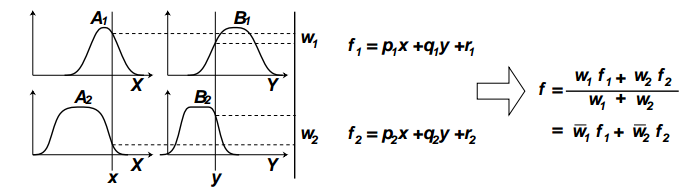
\includegraphics[scale=0.5]{images/TSK_Modell.png}
\caption{Inferenzschritt eines TSK-Modells \cite{Jang:93}}\label{TSK_Modell}
\end{figure}

In der Abbildung \ref{TSK_Modell} wird ein Model mit zwei Eingangsgrößen und zwei Fuzzy-Mengen pro Eingabe dargestellt. Die Regelbasis besteht aus zwei Regeln. Die Fuzzy-Mengen werden durch die Glockenfunktion berechnet. Die Variablen $w_1$ und $w_2$ liefern die Regelaktievierungen für die Regeln mit entsprechenden Indexen. Das Endergebnis ergibt sich aus der oben definierten Funktion \ref{TSK_defuzz}.

%Unsicher ob ich darauf eingehen soll

%Die Gliederung h�ngt nat�rlich vom Thema und von der L�sungsstrategie ab. Als n�tzliche
%Anhaltspunkte k�nnen die Entwicklungsstufen oder - schritte z.B. der Softwareentwicklung betrachtet werden. N�tzliche Gesichtspunkte erh�lt und erkennt man, wenn man sich
%\begin{itemize}
%  \item in die Rolle des Lesers oder
%  \item in die Rolle des Entwicklers, der die Arbeit z.B. fortsetzen, erg�nzen oder pflegen soll,
%\end{itemize}
%versetzt. In der Regel wird vorausgesetzt, dass die Leser einen fachlichen Hintergrund haben - z.B. Informatik studiert haben. D.h. nur in besonderen, abgesprochenen F�llen schreibt man in popul�rer Sprache, so dass auch Nicht-Fachleute die Ausarbeitung prinzipiell lesen und verstehen k�nnen.
%
%Die �u�ere Gestaltung der Ausarbeitung hinsichtlich Abschnittformate, Abbildungen, mathematische Formeln usw. wird in \hyperref[Stile]{Kapitel~\ref*{Stile}} kurz dargestellt.











%% KI Kapitel
\section{Künstliche Neuronale Netze} \label{ANN}

Künstliche Neuronale Netze (engl. artificial neural networks) sind Systeme, die auf dem Gehirn von Tieren und Menschen basieren und besteht aus endlich viele Einheiten, Neuronen. Der Datenaustausch geschieht über gerichtete Verbindungen zwischen den Neuronen. Forscher beschäftigen sich mit Neuronalen Netzen aus unterschiedlichen Gründen. In der Biologie simulieren Forscher diese, um sich den Prozess des Lernens und weitere Mechaniscmen zu untersuchen. In der Informatik wird aber versucht, die Lernfähigkeit des Gehirns nachzubilden und auszunutzen.

In den folgenden Kapiteln wird zuerst auf den Neuronen sowohl in der Biologie als auch in der Künstliche Intelligen eingegangen. Weiterhin werden die Eigenschaften von Neuronalen Netzen erklärt. Zum Schluss stelle ich den Gradientenvarfahren vor, anhand dessen diese Netze lernen.

\section{Biologische Grundlagen}

Das tierische Gehirn leitet jede einzelne Aktivität in dem Körper eines Tieres, inklusive die Verarbeitung von Daten. Laut \cite{GEHIRN:12} besteht das Gehirn aus 86 Milliarden Neuronen, die in Cliquen verbunden sind. Neuronen in einer Clique komunizieren untereinander, indem sie Signale über ihre Axone weiterleiten und Signale über ihren Dendrit empfangen. Eine Verbindung zwischen Neuronen existiert, wenn die Axonterminale eines Neurons den Dendrit eines anderen berührt. Zur Veranschaulichung ist den Aufbau eines Neurons in Abbildung \ref{neuron} gegeben. Jeder Signal wird in dem Soma verarbeitet und durch die Axone weitergeschickt.

\begin{figure}[!htbp]
	\centering
	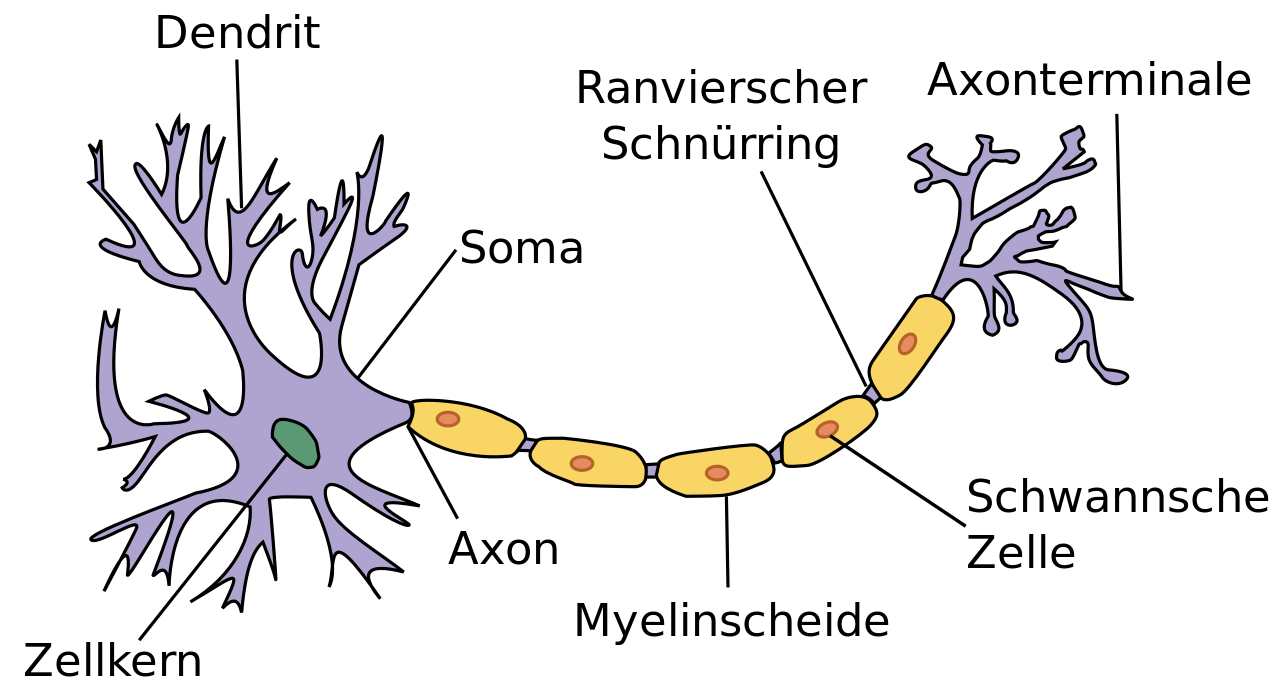
\includegraphics[scale=0.2]{images/Neuron_(deutsch)-1.png}
	\caption{Neuron \cite{NWIKI:19}}\label{neuron}
\end{figure}

Auf dem selben Prinzip funktionieren auch Neuronen in Künstlichen Neuronalen Netzen (KNN). Im folgenden Kapitel wird mehr darauf eingegangen. \cite{NWIKI:19} \cite{GEHIRN:12}

\subsection{Neuron in Künstlichen Neuronalen Netzen}

Neuronale Netze sind streng genommen gerichtete Graphen, wo jeder Knoten ein Neuron ist und jede Kante eine Verbindung zwischen Neuronen beschreibt. Die Neuronen können in drei Gruppen, oder auch als Schichten (\textit{engl.} Layers) bekannt, unterteilt werden - Eingabe-, Ausgabe- und versteckte Neuronen. Die Ein- und Ausgabeknoten sind die Einheiten, die mit der Umgebung verbunden sind, dabei ist klar welche Knoten was sind. Die übrigen Elemente werden in dem Netz eingebaut und kommunizieren nur mit anderen Neuronen. Daraus ergibt sich auch ihren Namen ``versteckt''.

Jede Verbindung zwischen Neuronen in KNN erhält ein Wert. Der Verbindungswert wird meistens als Gewicht bekannt. Bei einem Gewicht von 0 existiert keine Verbindung zwischen Neuronen. In einem KNN werden nur die Gewichte gelernt, während die Neuronen nur eine mathematische Funktion beschreiben. Eine übliche Repräsentation der Gewichte ist die Matrix \ref{knnmat}.

\begin{align}
\centering
\bordermatrix{ 	
	& u_1 			& u_2			 & \dots & u_r			    \cr
	u_1    & w_{u_{1}u_{1}} & w_{u_{1}u_{2}} & \dots & w_{u_{1}u_r}		\cr
	u_2	   & w_{u_{2}u_{1}} & w_{u_{2}u_{1}} & 	     & w_{u_{2}u_{1}}	\cr
	\vdots & \vdots	      	& 			     &       & \vdots			\cr
	u_r    & w_{u_{r}u_{1}} & w_{u_{r}u_{2}} & \dots & w_{u_{r}u_r}  	\cr 
}
\label{knnmat}
\end{align}

Die Beziehungen zwischen Neuronen aus zwei Schichten wird außerdem ganz gut in der Matrix dargestellt. Sie ist von oben nach rechts zu lesen, also die Spalten sind es dem Neuronen zugeordnet, aus denen die Verbindungen ausgehen. Das heißt der Knoten $u_1$ hat eine Verbindung zu sich selbst und dem Neuron $u_2$ und die Gewichtwerte sind entsprechend $w_{u_{1}u_{1}}$ und $w_{u_{1}u_{2}}$. Die Darstellung als Matrix erlaubt es alle mathematischen Operationen durchzuführen, indem der Ausgabe eines Neurons, oder die Eingabe aus der Umgebung, rechts an der Matrix dranmultipliziert. \cite{CIKruse:15} \cite{NFMBothe:98} \cite{SCTemassi:01} \cite{CISCNFI:98}

\section{Lernen} % s. 58 Book 2; s.40 Computational Intelligence s. 21
Die erstaunlichste Eigenschaft Neuronaler Netze ist ihre Möglichkeit, eine Aufgabe, bzw. Fähigkeit, zu erlernen. Gewichtswerte und/oder weitere Parameter unterliegt Änderungen nach jeder Iterationsschritt während des Lernprozesses. In Bezug auf dem Iterationsschritt wird es zwischen ``Offline-'' und ``Onlinelernen'' unterschieden. Außerdem unterscheidet man zwei weiteren Gruppen in der Lernmethode eines Neuronalen Netzes - überwachtes (\textit{engl.} supervised) und unüberwachtes (\textit{engl.} unsupervised) Lernen. Demnächst werden die Begriffe einzeln untersucht. Danach werden nur beaufsichtigte Algorithmen vorgestellt, da die relevant für mein Projekt sind. Zum Schluss werden die Offline- und Online-Lernverfahren vorgestellt, die insgesammt drei sind.  \cite{SCTemassi:01} \cite{CIKruse:15} \cite{NFSC:97} %Nach jedem Schritt können Gewichtswerte und/oder weitere Parameter optimiert werden.

\subsection{Unsupervised Learning}
Unsupervised Learning (\textit{deutsch} unbeaufsichtigtes Lernen) besteht immer noch eine Ein-/Ausgabe beziehung, jedoch wird kein Fehlerfunktion eingesetzt. In diesem Fall muss das Netz Mustern aus den Ein-/Ausgabepaare erkennen und zusammengruppieren.

\subsection{Supervised Learning}

Unter Supervised Learning versteht man den Verfahren, bei dem das Netz anahand von Ein-/Ausgabepaare trainiert wird. Das Lernenprozess beinhaltet die allmäliche Anpassung der Gewichtparametern bei jedem Iterationsschritt, so dass bei gegebener Eingabe $x$ der Fehler, der aus der Ausgabe und dem Erwartungswert berechnet wird, minimiert wird. Die Fehlerfunktion wird in vielen Fällen auch als ``Kritiker'' und das Modell als ``Kritisierender'' bekannt. Ein Speziallfall des überwachtes Lernen ist ``reinforcement Learning''. In dem Lernverfahren wird jede Berechnung ``richtig'' oder ``falsch'' bewertet, ohne dass ein Fehler unbedingt berechnet wird. \cite{SCTemassi:01} \cite{CIKruse:15} \cite{NFSC:97}

\subsubsection{Least Mean Square Method}
Die Kleinste Quadrate Methode (\textit{engl.} Least Mean Square Method) wurde von den B. Widrow und M.Hoff für ein Projekt namens ADALINE oder ADAptive LINear Element entwickelt. Die Methode versucht die Fehlerrate mit dem Gradientenverfahren zu verringern. Die Fehlerrate wird mit dem Mean Squared Error (MSE) geteilt durch die Anzahl der Elementen im Trainingsdaten berechnet. Die Formel ist gegeben:

\begin{align}
E(w) = \frac{1}{2} \sum_{i=1}^{m}(d_i - y_i)^2 \label{MSE}, 
\end{align}

wobei $w$ ist der Gewichtsvektor, und $d_i$ und $y_i$ entsprechend - Erwartungs- und Ausgabewert. Die Ableitung der Funktion ergibt den nächsten Iterationsschritt:

\begin{align}
w^{t+1} = w^t + \mu(d_k^t - y_k^t)x_k^t.
\end{align}

Die Konstante $\mu$ kontrolliert die Konvergenz und Stabilität, \textbf{w} und textbf{x} sind Gewichtsvektor und Eingabe. Der Schritt wird durch den Exponent $t$ bestimmt - $t+1$ ist der nächste Schritt. Solange die Konstante entsprechend gewählt wird, konvergiert der Verfahren und der gesuchte Gewichtvektor kann gelernt werden. \cite{SCTemassi:01}

\subsubsection{Backpropagation Algorithm}
Der Backpropagation Algorithmus, oder auch als Gradient Descent bekannt, wurde laut \cite{SCTemassi:01} am Ende der 70er Jahren von Paul J. Warbos entwickelt. Dieses Verfahren hat die Interesse an Neuronalen Netzen wiederbelebt.

Der Algorithmus ist der bekannteste Lernalgorithmus für beaufsichtigtes Lernen. In dem Verfahren stecken zwei wichtige Konzepte. Zum einen liegt der Feedforwardphase vor, die dann folgendes Verhalten beschreibt: die Eingabe-/Erwartungswerte dem Neuronalen Netz gegeben werden und anschließend eine Ausgabe berechnet wird. Danach wird der Fehler berechnet, für den eine bestimmte Fehlerfunktion verwendet wird, z.B. der Mean Squared Error (siehe Gleichung \ref{MSE}). In der zweiten Phase, auch Rückwertsphase genannt, werden die Knoten rückwerts anfangend von der Ausgabe- über die versteckten Schichten bis zum Eingabeschicht angepasst. Das Ziel der Rückwertsschritt ist es den Fehlre zu minimieren. Hinter dem Verfahren stecken einfache Mathematische Operationen, wurde aber in dieser Ausarbeitung nicht betrachtet. In dem Buch \cite{SCTemassi:01} wird jedoch eine sehr ausführliche Beschreibung des Algorithmus in Schritten angegeben, welche auch hier figuriert.

\begin{enumerate}\label{BPA}
	\item Die Gewichte werden zufällig initialisiert.
	\item Eine Ein-/Ausgabe paar wird dem Netz vorgestellt.
	\item Liefer die Ausgabe des Netzes.
	\item Berechne die Fehlerrate (z.B. durch die Mean Squared Error \ref{MSE}).
	\item Beginnend mit der letzten Schicht berechne den Wert der Ableitung $\delta_j$ rückwerts.
	\item Passe die Gewichte nach in dem Netz.
	\item Wiederhole ab 2. Schritt für angegebene Anzahl an Iterationen, oder bis die Fehlerrate kleiner als ein Betrag wird.
\end{enumerate}

% Hier das Algorithmus, wie es im Buch figuriert, angeben

\subsection{Schlüsse}

Es werden zwei Bibliotheken für Neuronale Netze berücksichtigt - Tensorflow und SciKit. Biobliotheken sind in der Regel sehr ähnlich. In diesem Fall bieten die betrachteten APIs die nötigten Funktionalitäten, um das Projekt umzusetzen. Jedoch das Ursprüngliche Gedacht war, dass ich die erstellten Neuronalen Modelle in C++ exportiere. Das würde erfordern, dass eventuell das ANFIS-Model mit Hilfe von andere Bibliotheken gegenüber C++ kompilieren müsste. Der Grund, warum ich dann zu Tensorflow geneigt habe, ist, weil Tensorflow geschriebene Modelle, einfach in Dateien zu exportieren sind. Was wiederum mich erlaubt das Model in C++ ohne weiteres zu importieren.

%% Neuro Fuzzy








\section{Neuro-Fuzzy-Systeme}

Im vorletzten Kapitel wurden zwei Arten von Fuzzy-Systeme, oder Reglern, vorgestellt. Solche Systeme werden in der Praxis öfters mit Konzepte aus der Künstliche Intelligenz kombiniert. Zum einen bietet sich Kombinationen mit Neural Networks \ref{ANN}, Evolutionäralgorithmen und vielen weiteren. Im folgenden Kapitel wird besonders die Kombination mit Neuronalen Netzen untersucht. Die Zusammenarbeit von Fuzzy-Reglern und Neuronalen Netzen ist atraktiv, weil die Interpretierbarkeit von Fuzzy-Systeme mit den Lernmöglichkeit von Neuronalen Netzen effektiv zu verbinden ist. In den nächsten Unterkapiteln werden zwei Arten von Modelle mit jeweils einer Beispielstruktur - Modelle für feste Lernaufgaben und solche mit verstärkendem Lernen. Die Modelle werden außerdem in der Literatur als Neuro-Fuzzy-Systeme, bzw. Neuro-Fuzzy-Regler, bezeichnet. \cite{CIKruse:15}
\section{Neuro-Fuzzy-Regler}

Neuro-Fuzzy-Regler, oder Neuro-Fuzzy-Systeme, sind Modelle, bei denen konzeptionelle Teile von Neuronalen Netzen und Fuzzy-Systeme kombiniert werden. Das Ziel dieser Reglern ist es das beste aus beiden Welten zu kombinieren - Lernbarkeit von Neuronalen Netzen und Interpretierbarkeit von Fuzzy-Systeme. Außerdem bietet Fuzzy-Systeme die Möglichkeit Vorwissen einzubrigen, was hingegen die Lernzeit der Neuronalen Netze verkürzt. Am Ende des Lernprozesses erhält man ein Modell, dessen Regelungsstragie interpretierbar ist und dessen Regelung überprüft und eventuell noch angepasst werden können \cite{CIKruse:15}. Demnächst werden zwei Arten von Neuro-Fuzzy-Modelle, die unterschiedliche Anwendungsfälle haben.

\subsection{Modell f\"{u}r feste Lernaufgaben}
%(Muss Änderungen unterliegen)

Neuro-Fuzzy-Modell für feste Lernaufgaben versuchen, Fuzzy-Mengen und, bei TSK-Modelln, die Parameter der Ausgabefunktion unter Einreichung einer Mengen von Ein-/Ausgabe-Tupeln zu optimieren. Diese Modell sind genau dann sinnvoll, wenn schon eine Fuzzy-Regelbasis vorliegt. Die Regelbasis unterliegt infolge des Lernens eine Verarbeitung, die als Ziel eine Optimierung hat. %Dafür sind geieignete Ein-/Ausgabedaten gebraucht.

Ein weiteres Anwendungsbeispiel ist bei bereits existierender Regelbasis, dass dieser mit einer neuen ausgetauscht wird. Falls die Basis schon errechnete Werte geliefert hat, können diese zusammen mit den zugehörigen Eingabewerten dem Neuro-Fuzzy-System zum Lernen gegeben werden. Am Ende erhält man eine optimierte Fuzzy-Regel-Basis, die die alte Basis ``ersetzt''.

Falls es keine angemessene Lernaufgabe bereits gegeben ist, dann eignet sich dieses Verfahren nicht. Es existieren natürlich Ansätze, die es ermöglichen, einen initialen Regelbasis aus Eingabedaten zu erstellen. Ein solcher Verfahren wird später noch vorgestellt.

Folglich wird ein Beispiel von einem Modell, das sich für feste Lernaufgaben eignet, vorgestellt. Es geht nämlich um das ANFIS-Modell.

\subsubsection{Das ANFIS-Modell}

Im Frühjahr von 1993 wurde das Neuro-Fuzzy-System ANFIS (Adaptive Neuro-Fuzzy Inference System oder Adaptive Network-based Fuzzy Inference System) entwickelt. Das Modell wurde in mehrere Software-Pakete schon eingesetzt. Die ANFIS basiert auf einer hybriden Struktur, sodass es sowohl als ein Neuronales Netz, als auch als ein Fuzzy-System interpretiert werden kann. In dem System sind Regeln angelegt, die nach dem TSK-Modell definiert sind (Takagi-Sugeno-Kang-Reglern \ref{TSK}). Die Abbildung \ref{ANFIS_Abb} zeigt einen Modell mit folgender Regelbasis:%(Abbildung hier zitieren aus Buch 2)

\begin{minipage}{\textwidth}

\begin{center}
	$\newline$
	$R_1$: Falls $x_1$ ist $A_1$ und $x_2$ ist $B_1$, dann ist $y$=$f_1$($x_1$,$x_2$)\\
	
	$R_2$: Falls $x_1$ ist $A_1$ und $x_2$ ist $B_2$, dann ist $y$=$f_2$($x_1$,$x_2$)\\
	
	$R_3$: Falls $x_1$ ist $A_2$ und $x_2$ ist $B_2$, dann ist $y$=$f_3$($x_1$,$x_2$),
\end{center}
\end{minipage}
dabei sind $A_1$, $A_2$, $B_1$ und $B_2$ linguistische Termen, die den entsprechenden Fuzzy-Mengen $\mu_i^{(j)}$ zugeordnet sind. Die Funktionen $f_i$ sind linear und sehen wie folgt aus (siehe \ref{FDF}):
\begin{equation}
f_i(x_1, x_2) = p_0^{i} + p_1^{i}\cdot x_1 + p_2^{i}\cdot x_2
\end{equation}

Der Konklusionsfunktion $f_i$ entspricht die Regel $R_i$. Somit hat jede Regel eine eindeutige Ausgangsfunktionen mit eindeutigen Parametern $p_0^{i}, p_1^{i}, p_2^{i}$.

Die Ausgabe eines ANFIS-Modells berechnet sich genau so wie ein TSK-Modell (siehe \ref{FDF}). %Zuerst wird der Zugehörigkeitsgrad einer Regel mit dem entsprechenden Konklusionsfunktion multipliziert. WeiterhinAnschließend normiert man das Resultat  summiert man das Resultat aus allen Regeln und teilt die Summe durch die Summe aller Anktivierungsgraden. 
Für den genannten Beispiel lautet die Ausgabe:
\begin{align}
f = \dfrac{\sum_{i}^{3} \tilde{w_i}\cdot f_i(x_1, x_2)}{\sum_{i}^{3} \tilde{w_i}}
\end{align}

Der ANFIS-Ansatz besteht aus 5 Schichten. Die Abbildung \ref{ANFIS_Abb} veranschaulicht die Struktur.

\begin{figure}[htbp]
	\centering
	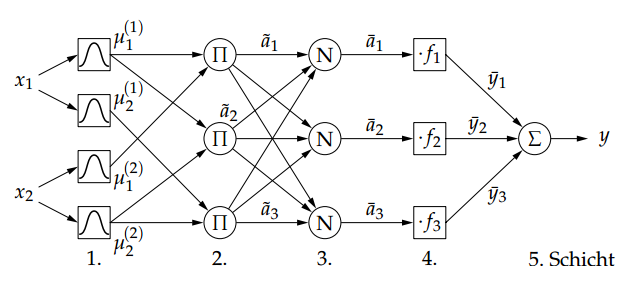
\includegraphics[scale=0.5]{images/ANFIS_Abb.png}
	\caption{ANFIS-Model \cite{CIKruse:15}}\label{ANFIS_Abb}
\end{figure}

In der \textbf{ersten Schicht} werden die Eingabewerte eingereicht und entsprechend die Zugehörigkeiten zu den Fuzzy-Sets ausgegeben. Weiterhin werden in der \textbf{zweiten Schicht} die Aktivierungswerte jeder Regel ausgewertet. Die Neuronen werden mit $\prod$ gekennzeichnet. Einzelnen Fuzzyzugehörigkeitswerte werden mittels Operatoren kombiniert, um die Aktivierungsgrad jeder Regel zu berechnen. Hier dürfen Operatoren zur Verknüpfung von Fuzzy-Mengen eingesetzt werden, üblicherweise der UND-Operator (siehe \ref{AND}). Die Gleichung \ref{eq3_3} ergibt die Berechnung bei gegebener UND-Verknüpfung:

\begin{equation}\label{eq3_3}
\tilde{w}_i = \prod \mu_i^j(x_j)
\end{equation}

Die Variable $\tilde{w}_i$ ergibt die Aktivierung, oder Erf\"{u}llungsgrad, des Regels $R_i$ und $\mu_i^j$ ist die $j.$ Zugehörigkeitsfunktion in der Regel $R_i$.

Im \textbf{dritten Schicht} findet die Normalisierung aller Aktivierungswerte $\tilde{w}_i$ statt. Mit einfachen Worten wird der Beitrag berechnet, den jeder Regel für den Gesamtausgabe beiträgt. Nach der Normalisierung erhält man Aktivierungsgrößen zwischen $0$ und $1$. Die Gleichung \ref{barwi} berechnet die normalisierten Werten für jeden Regel $R_i$:

\begin{equation}\label{barwi}
\bar{w}_i = \frac{\tilde{w}_i }{\sum_j \tilde{w}_j } 
\end{equation}

Im \textbf{vierten Schicht} berechnen die mit $N$ markierten Neuronen die gewichteten Ausgabewerte. Das ``Gewicht'' (Ergebnis) aus dem letzten Layer wird mit der entsprechenden Ausgabefunktion multipliziert:

\begin{equation}
\bar{y}_i = net_i = \bar{w}_i\cdot f_i(x_1, ..., x_n). 
\end{equation}

Im \textbf{fünften Schicht} steht ein einziges Neuron, der mit $\sum$ beschriftet ist. Im letzten Schicht berechet man die Ausgabe, indem alle Werte aus dem \textbf{vierten Schicht} zusammenaddiert werden:

\begin{equation}
y = y_{out} = \sum_i \bar{y}_i = \frac{\tilde{w}_i\cdot f_i(x_1, ..., x_n)}{\sum_j \tilde{w}_j}.
\end{equation}

Diese Struktur ähnelt sich der von TSK-Modell. Für die Optimierung von Parametern der Zugehörigkeitsfunktionen und Konklusionsfunktionen eignet sich der ANFIS-Ansatz.

Das ANFIS-Modell ermöglicht die Optimierung von Modellparametern - die Fuzzy-Mengen- und Ausgabefunktionsparametern. Diese können erlernt werden, wenn eine angemessene Lernaufgabe vorliegt. Außerdem muss eine ausreichende Menge von Ein-/Ausgabe-Werten zur Verfügung stehen. Es bieten sich mehrere Lernmethoden zur Optimierung der Parametern. Zwei davon sind Gradientenverfahren(analog zur Fehler-Rückpropagation-Verfahren aus Neuronalen Netzen) und die Kleinste-Quadrate-Methode. \cite{CIKruse:15} \cite{Jang:93}

\subsection{Modell mit verstärkendem Lernen}

Bei Modellen mit verstärkendem Lernen wird versucht, die Menge der Daten für das Lernen möglichst gering zu halten. Der Unterschied zwischen Modell mit verstärkendem Lernen und solchen für feste Lernaufgaben besteht darin, dass bei dem Erstgenannten keine Vorwissen bekannt werden müssen, was öfters der Fall sein kann. Es reicht nur, wenn im Laufe des Lernens angegeben wird, ob die Richtung der Optimierung sinnvoll ist.

Ein großes Problem beim verstärkendem Lernen besteht darin, vorzusagen, wie groß der Einfluss einer Regelaktion auf das Gesamtsystem ist. Dieses Problem wird als \textit{Credit Assignment Problem} bezeichnet.

Es existiert eine große Mengen von Modelln mit verstärkendem Lernen, alle aber basieren auf dem gleichen Prinzip. Das System wird zwei Teilsysteme aufgeteilt: zum einen der ``Kritiker''(das ``kritisierende'' System) und der Aktor(zuständig für die Anwendung und Abspeicherung der Regelungsstrategie). Der Kritiker ``äußert'' seine Meinung über den jetzigen Zustand unter Berücksichtigung der vorhergehenden Zustände und somit entscheidet der Aktor anhand der Bewertung, ob eine Korrektur der Regelbasis gemacht werden soll. \cite{CIKruse:15}  \cite{UNIMAG:97}

\subsubsection{Das NEFCON-Modell}

Ziel des NEFCON-Modell, Neuro-Fuzzy Control Modell, ist es, eine interpretierbare Fuzzy-Regelbasis mit möglichst kleinen Trainingsschritten zu erlernen. Das Modell unterscheidet sich von dem ANFIS, indem es erlaubt einen Regelbasis, ohne Vorwissen zu erlernen. Dieses Modell bietet natürlich auch die Möglichkeit, Vorwissen mitzubringen. Das heißt sowohl Fuzzy-Systeme mit vorhandenen Regelbasis, als auch solche mit unvollständiger Fuzzy-Regelbasis. Alle diese Vorteilen sprechen für das NEFCON gegenüber andere Modelle.

Das NEFCON-Modell basiert auf ein Mamdani-Regler. Zum Veranschaulichung wird hier einen kleinen Beispiel mit Grafik \ref{NEFCON_Abb} und Regelbasis gegeben: \cite{CIKruse:15}
\begin{minipage}{\textwidth}
	

\begin{center}\label{nef_regelbasis}
	$\newline$
	$R_1$: IF $x_1$ in $A_1^{(1)}$ AND $x_2$ in $A_1^{(2)}$, THEN y is $B_1$ \\
	
	$R_2$: IF $x_1$ in $A_1^{(1)}$ AND $x_2$ in $A_2^{(2)}$, THEN y is $B_1$ \\
	
	$R_3$: IF $x_1$ in $A_2^{(1)}$ AND $x_2$ in $A_2^{(2)}$, THEN y is $B_2$\\
	
	$R_4$: IF $x_1$ in $A_3^{(1)}$ AND $x_2$ in $A_2^{(2)}$, THEN y is $B_3$\\
	
	$R_4$: IF $x_1$ in $A_3^{(1)}$ AND $x_2$ in $A_3^{(2)}$, THEN y is $B_3$
	
\end{center} 
\end{minipage}

\begin{figure}[htbp]
	\centering
	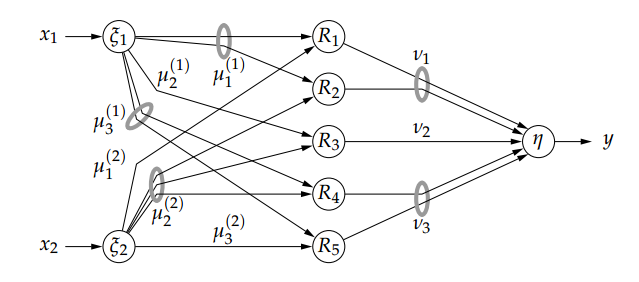
\includegraphics[scale=0.5]{images/nefcon_abb.png}
	\caption{NEFCON-Modell \cite{CIKruse:15}}\label{NEFCON_Abb}
\end{figure}

%\begin{align}

%\end{align}
% Hier Grafik einfügen

Das NEFCON-Modell basiert auf einem generischen Fuzzy-Perzeptron. Das Modell konnte in drei Schichten aufgeteilt werden. Die \textit{erste Schicht} besteht natürlich aus den Eingangsneuronen. Die ist eindeutig und will nicht weiter darauf eingehen. In der \textit{zweiten Schicht} befinden sich die inneren Neuronen, die die Regeln einer Fuzzy-System widerspiegeln. Im Beispiel sind insgesamt fünf Regeln gegeben. Die Fuzzy-Mengen $\mu_r^{(i)}$, die in Mehrere Regeln vorhanden sind, werden durch Ellipse zusammengeführt. Falls beim Lernen eine Anpassung an einem Gewicht durchgeführt werden soll, muss dies in allen Verbindungen gemacht werden, wo die Menge figuriert.

Der eigentliche Lernprozess besteht aus zwei Phasen. In der erste Phase wird versucht, eine Regelbasis erlernt zu werden. Diese Phase wurde weggelassen, falls schon eine existiert. Es lassen sich auch unvollständige sogar fehlende Regelbasen lernen. Für das Letztere ist ein weiterer Algorithmus erforderlich.

In der zweiten Phase findet die Optimierung statt. Dabei werden Fuzzy-Sets modifiziert oder selbst die Verbindungen zu den Regeln umgetauscht. In dem NEFCON-Modell wird als Bewertungsmaß, der ``Kritiker'', ein Fuzzy-Error verwendet. Damit die Optimierung optimal ausgeführt werden kann, sollte das Vorzeichen des Ausgabewertes bekannt sein. Darüber hinaus wird ein erweiterter Fuzzy-Error $E^*$ berechnet:
\begin{equation}\label{EFE}
E^* = sgn(y_{out})\cdot E(x_1, \ \ldots , \ x_n)
\end{equation}
\cite{CIKruse:15} \cite{UNIMAG:97}
\section{Erlernen einer Regelbasis}

Es existieren mehrere Algorithmen zum Erlernen von Regelbasis. Die Methoden können in drei Kategorien aufgeteilt werden: solche, die ohne vordefinierte Regelbasis startet; solche mit vollständiger Regelbasis und solche mit zufälliger Basis  starten. In den folgenden zwei Unterkapiteln werden Methode für die ersten zwei Kategorien vorgestellt. Bei den Methoden wird keine feste Lernaufgabe benötigt. Tatsächlich geht es darum, dass eine Initialbasis aufgebaut wird, ohne eine große Datenmenge mit optimalen Werten bekannt zu sein. \cite{CIKruse:15} \cite{UNIMAG:97}% Bis Hier drübergeguckt

\subsection{Top-Down- oder Reduktionsmethode zum Erlernen einer Regelbasis}

Zum Einen wird die Methode der Top-Down-Methode (in der Literatur auch als NEFCON I bekannt) genannt. Das Verfahren erfordt, dass eine vollständige Regelbasis vorhanden ist. Die Regelbasis beinhaltet auch widersprüchliche Regeln, die in Laufe des Prozesses ausgefiltert werden.

Der Prozess kann in zwei Phasen aufgeteilt werden. In der ersten Phase werden alle die Regeln eliminiert, die bei ihrer Ausgabe den falschen Vorzeichen aufweisen. Die auszufilternden Regeln werden mit der erweiterten Fuzzy-Fehler-Funktion (siehe \ref{EFE}) bestimmt. In der zweiten Phase werden Regeln mit identischer Prämisse zufällig ausgewählt. Folglich wird der Fehler für die bestimmte Regel berechnet. Zum Schluss wird die Regel ausgewählt, die die kleinste Fehlerrate aufweist. Die restlichen Regeln werden verworfen.

Eins der Nachteile der Top-Down-Methode ist die Aufwändigkeit, weil es mit einer großen Regelbasis gestartet wird. Das nächste Verfahren ist das Gegenteil von Top-Down-Methode, zwar Bottom-Up-Methode. \cite{CIKruse:15}


\subsection{Bottom-Up- oder Eliminationsmethode zum Erlernen einer Regelbasis}

Der Bottom-Up-Algorithmus beginnt mit einer leeren Regelbasis. Jedoch muss eine initiale Aufteilung(Intervall) der Ein- und Ausgabewerten gegeben sein. Analog zur Top-Down besteht diese Methode auch aus zwei Phasen. 

Erste Phase beginnt mit der Bestimmung der Prämisse für die Regeln. Der Prozess evaluiert jede Fuzzy-Menge mit bestimmten Eingaben und die Mengen, die den höchsten Zugehörigkeitsgrad aufweisen, werden ausgewählt. Aus den ausgewählten Fuzzy-Mengen werden neue Regeln gebaut. Danach versucht der Algorithmus eine geeignete Ausgabe aus dem aktuellen Fuzzy-Fehler zu ``raten''. Dabei wird vorausgesetzt, dass Eingaben mit ähnlichen Fehlerwerten ähnliche Ausgaben liefern.

In der zweiten Phase werden die Fuzzy-Mengen in den Konklusionen optimiert. Dabei werden nicht die Parametern der Konklusionen angepasst, sondern bei Bedarf die Fuzzy-Menge durch eine andere ersetzt.

Wegen des inkrementellen Lernen lässt sich einfach Vorwissen in dem Regelbasis einführen. Bei den Fällen mit unvollständigen Regelbasen werden passende Regeln hinzugefügt. Das Verfahren garantiert jedoch nicht, dass immer eine geeignete Regelbasis aufgebaut wird. Aus diesem Grund ist es empfohlen, dass die Regelbasis manuell am Ende des Lernens überprüft und entsprechend angepasst wird. \cite{CIKruse:15} \cite{UNIMAG:97}

\section{Optimierung der Regelbasis}

Die Optimierung bei NEFCON verwendet die Methode ``Back Propagtion Method'', oder Rückpropagationsmethode. Der Fehler wird rückwirkend durch das Netz geführt und lokal bei jeder Fuzzy-Menge angewendet.

Eine Änderung darf sowohl in den Prämissen, als auch in den Konklusionen. Es wird das Prinzip des verstärkenden Lernens angewendet. Das bedeutet, dass für jede Änderung eine Fuzzy-Menge entweder ``bestraft'' oder ``belohnt'' wird. Bestrafung und Belohnung werde in Änderungen wie Verschiebung, Vergrößerung oder Verkleinerung des Bereichs einer Fuzzy-Menge ausgedrückt. Änderungen werden entsprechend iterativ in Beziehung zum Fuzzy-Fehler gemacht. \cite{CIKruse:15} \cite{UNIMAG:97}

\section{Schlussworte}

% Zusammenfassung der zwei Methoden,
Die Methoden unterscheiden sich in ihrem Kern kaum. Beide Architekturen besitzen entsprechend Vorteile und Nachteile. Der größte Unterschied liegt in der Ausbau ihrer Struktur. ANFIS basiert auf TSK-Modellen, währen NEFCON auf die Mamdani-Reglern. Beide Modelle bieten sie sich gut für das Lernen von Fuzzy-Systeme, jedoch entspricht nur das ANFIS meinem Anwendungsfall - Optimierung von TSK-Modelle.